\chapter{Introduction}
\section{Problem statement}
Due to the damaging environmental effects of using fossil fuels in the transport sector, national and 
international targets have been set in order to reduce global CO\textsubscript{2} emissions.
In the UK for example, there is a plan to completely ban the sales of new conventional petroleum vehicles 
by as early as 2040. 
\cite{DepartmentforEnvironment2017} 
One proposed solution is further adoption of fuel cells and other energy generation methods which utilize
hydrogen as a carbon free energy source. 

Despite the fact that the technology for hydrogen powered fuel cells has existed since the early 1960’s their application has been limited to providing 
power for space missions and other niche applications. It wasn’t until the late 90’s where developments 
in lowering the platinum catalyst loading and the production of thin film electrodes drove the cost of fuel 
cells down to a level where they were a commercially viable option. As of 2017, a number of auto 
mobile manufacturers including Toyota,\cite{Toyota2015} Hyundai, \cite{Hyundai2015} Honda \cite{Honda} 
and Daimler \cite{Mohrdieck2014} now offer hydrogen vehicles commercially. It is also becoming 
increasingly possible to retrofit a petroleum vehicle to run off hydrogen.\cite{FCell2016} 
Many countries both in the EU, and globally have ambitious hydrogen infrastructure plans over the next 
10 years. This is in an effort to become less reliant on importing fossil fuels, increase their energy security,
and transition to a carbon free energy system.

The development of the hydrogen economy is still in its infancy ,  however several 
countries are aiming to employ sizable hydrogen fuelling infrastructures over the next few decades. 
National reports state that Europe’s position in 2030 will be: UK - 1,100 hydrogen refuelling stations
and 1.6 million fuel cell vehicles \cite{UKH2Mobility2013} France – 600 hydrogen refuelling stations 
and 0.8 million fuel cell vehicles \cite{Summerton2015}, Germany – 1,180 hydrogen refuelling stations 
\cite{Hayter2014} 
and 1.8 million fuel cell vehicles  and the Netherlands – 200 hydrogen refuelling stations and 0.2 
million fuel cell
vehicles. \cite{Hayter2014} The fuel cell system in a hydrogen vehicle can easily degrade if even 
parts-per-billion to parts-per-million level of some impurities are present in the hydrogen. 
Therefore, it is imperative that hydrogen purity, and techniques for verifying the purity, 
are adequate to ensure customers vehicles are not inadvertently damaged by fluctuations in hydrogen 
composition. 

International standards dictate that it is mandatory for all hydrogen suppliers to prove that their 
product is pure enough to prevent degradation of fuel cell components. The international standard ISO
14687-2:2012 \cite{InternationalStandardISO14687-2:20122012} shown in Table \ref{tab:1} specifies the 
maximum impurity levels of 13 impurities that are 
permissible in fuel cell hydrogen. ISO 14687-2:2012 includes some challenging hydrogen purity 
specifications mainly due to the low limits of detection of standard techniques used to measure the 
compounds included in the standard. 

\begin{table}[]
    \caption{Concentration limits for ISO-14687 impurities}
    \centering
    \begin{tabular}{@{}cc@{}}
    \toprule
    \textbf{Characteristics}                  & \textbf{Regulation}    \\ \midrule
    Minimum mole fraction of hydrogen         & 99.97\%                \\
    Total non-hydrogen gases                  & 300 µmol mol-1         \\ \midrule
    \multicolumn{2}{c}{\textbf{Maximum concentration of individual components}} \\ \midrule
    Total Hydrocarbons (Methane basis)        & 5 µmol mol-1           \\
    Water                                     & 2 µmol mol-1           \\
    Oxygen                                    & 5 µmol mol-1           \\
    Helium                                    & 300 µmol mol-1         \\
    Carbon dioxide                            & 2 µmol mol-1           \\
    Carbon monoxide                           & 0.2 µmol mol-1         \\
    Total sulphur compounds (H\textsubscript{2}S basis)       & 0.004 µmol mol-1       \\
    Formaldehyde                              & 0.01 µmol mol-1        \\
    Formic acid                               & 0.2 µmol mol-1         \\
    Ammonia                                   & 0.1 µmol mol-1         \\
    Total halogenated compounds               & 0.05 µmol mol-1        \\
    Maximum particulate concentration         & 1 mg/kg                \\ \bottomrule
    \end{tabular}
    \label{tab:1}
\end{table}

Existing hydrogen purity laboratories are unable to perform traceable analysis to ISO 14687 
specifications because appropriate methods and standards have not been developed. The consequence 
of this is that hydrogen suppliers cannot provide evidence that their fuel meets the International 
Standard and therefore are not permitted to supply hydrogen. Of the 13 gaseous impurities listed in 
ISO 14687-2, there is no single method for measuring all impurities. Laboratories must therefore use 
several instruments to perform such an analysis.  In 2015 Murugan et al published a review of methods 
for analysing the purity of fuel grade hydrogen \cite{Murugan2015}. They concluded that in order for a single 
laboratory to provide full hydrogen analysis to ISO 14687-2 specifications it would need to comprise 
a variety of instruments including GCs, FTIR and CRDS. The capital cost of purchasing the gas 
analysers to perform analysis on the measurable impurities in a hydrogen sample can amount to 
>€500,000 \cite{Murugan2015} and hence performing analysis would be out of reach for many of the smaller 
laboratories. 

While the impurities listed in ISO 14687-2 are specified at extremely low amount fractions, 
many can be analysed at higher amount fractions through the use of cheap and routine gas 
analysers such as GC-MS. A potential solution to this would be to increase the concentration 
above the limit of detection of one of these cheaper analysers. These techniques are referred 
to as enrichment or pre-concentration. The most commonly used technique for pre-concentration 
of hydrogen fuel samples is referred to as ‘Hydrogen Impurity Enrichment’.  This method involves 
passing the sample through a palladium or palladium alloy membrane which is heated to 400\textdegree C. 
Palladium as a membrane material only allows the passage of hydrogen, and as hydrogen leaves the system, 
the impurities remain, increasing in time as more hydrogen permeates through the membrane.
This increase in concentration is referred to as the enrichment factor and. 
Once the enrichment is complete the sample can then be analysed at these higher concentrations, 
and using the enrichment factor, the original composition of the sample can be found. 

In order for these devices to provide accurate results the behaviour of the membrane material, and its interaction with any impurities present in the hydrogen same, must be properly understood.  


\section{Research Background}
\subsection{Hydrogen Production}
Hydrogen production refers to a range of industrial processes for generating hydrogen. 
Since there are no natural reserves of hydrogen all hydrogen must be obtained through one of these methods. 
The most important factor for determining the feasibility of a hydrogen production process is the primary 
source of energy that is used. Currently the options for this are nuclear energy in the form of heat, 
renewable energy in the form of heat, electricity, or light, or fossil fuels. 
Currently the primary sources of hydrogen are from steam reforming of methane and other hydrocarbons which 
in total accounts for 96\% of global hydrogen production, with electrolysis of water accounting for the 
remaining 4\%.
\subsubsection{Hydrogen from fossil fuels and hydrocarbons}
Fossil fuels are the most dominant source of hydrogen production and there are a number of processes which 
utilize fossil fuels to produce hydrogen. The most popular and therefore the ones which will be discussed 
are steam methane reforming, hydrocarbon decomposition
\paragraph{Steam Methane reforming}
is the conventional and most economical method for producing hydrogen, and it has been predicated by the 
IEA that this trend will continue despite the emergence of other hydrogen production methods. 
Steam methane reforming occurs through a two-step chemical process. If another hydrocarbon other than 
methane is being used it must first be pre-reformed into methane as shown in equation \ref{eq:1}

\begin{equation} \label{eq:1}
    C_n H_m + H_2 O \rightarrow nCO +(\frac{n+m}{2})H_2 
\end{equation}
\begin{equation}\label{eq:2}
    CH_4 + H_2 O \rightarrow CO + 3H_2 \quad \Delta H_{298K}^o = +205 kJ/mol
\end{equation}
\begin{equation}\label{eq:3}
    CO+ H_2 O \rightarrow CO_2 + H_2 \quad \Delta H_{298K}^o = -41 kJ/mol
\end{equation}

Equation \ref{eq:2} takes place in a reactor operating at 700-850\textdegree C, at pressures of 3-25 bar, 
and in the presence of a nickel based catalyst. 
The result of this step is a mixture of CO and H\textsubscript{2}, commonly referred to as syngas. 
This syngas is used as a feedstock for the reaction shown in equation \ref{eq:3} known as water gas 
shift in order to produce greater hydrogen yields.  
This step is carried out in a two-step reaction. 
An initial high temperature stage at 350\textdegree C which converts majority of the syngas to 
CO\textsubscript{2} and hydrogen, and a final low-temperature step which operates at 250\textdegree
C which utilizes a catalyst with higher activity to minimise the remaining CO\textsubscript{2}. 
The final product will be a mixture of CO\textsubscript{2} and H\textsubscript{2}.  

A number of separation steps are utilised in order to prevent impurities from contaminating the 
resulting gas mixture. The traditional separation step is pressure swing adsorption (PSA) which takes 
advantage of adsorption of gaseous molecules onto a molecular sieve at high pressures. Hydrogen purities 
of ~99.9\% are achievable using this method however the cost is high and typically contributes to around 
20-30\% of the total production cost. The other main separation step is desulphurization which uses a 
combination of CoMo and ZnO catalysts in series at 450-550\textdegree C to remove sulphur. 
This step is essential to ensure sulphur is not present in the gas exit stream and also to ensure catalyst 
poisoning does not occur at any point in the process. 

\paragraph{Hydrocarbon decomposition}
is a process by which hydrocarbon molecules are converted into solid carbon and hydrogen. 
This reaction is typically operated either thermally or by creating a plasma. 
Both methods require a metallic catalyst such as nickel or iron. 
The reaction is shown in equation \ref{eq:4}

\begin{equation}\label{eq:4}
    C_x H_2x+2 \rightarrow xC + (x+1)H_2
\end{equation}

An advantage of this process is that the only feedstock is the hydrocarbon, so presuming that the feedstock 
is sufficiently pure this method of hydrogen production should remove the needs for further downstream 
processing. 
The main disadvantage of this method is the since solid carbon is the main by-product the catalyst will 
easily be deactivated and will require regular maintenance.
\subsubsection{Hydrogen from water}
\paragraph{Thermal decomposition of water}
is the process of splitting water into hydrogen and oxygen at temperatures of 2000\textdegree C, 
this can be lowered under the presence of a nickel or iron based catalyst. 
Due to the high energy demand for this production method water splitting is not a feasible method of 
commercial hydrogen production.

\begin{equation}
    H_2 O \rightarrow H_2 + \frac{1}{2} O_2  \quad \Delta H_{298K}^o = +286 kJ/mol
\end{equation}

\paragraph{Electrolysis}
is the second most popular method for producing pure hydrogen after SMR. 
This method uses an electric current to split water into hydrogen and oxygen. 
The main competitive advantage of electrolysis is that they are modular and highly scalable, 
allowing hydrogen to be produced in a distributed manner. 
The main input to the process is electricity and if this electricity is produced using renewable sources 
then the process can be considered carbon neutral. 
This is further incentivised by the increasing price of natural gas and the decreasing price of electricity, 
which some predict will result in electrolysis becoming more economically feasible than SMR in the future. 
\begin{equation}
2H_2 O +  2e^- \rightarrow H_2 + 2OH^-
\end{equation}
\begin{equation}
2OH^- \rightarrow \frac{1}{2}O_2+ H_2 O + 2e^-
\end{equation}


\subsection{Hydrogen impurities in the supply chain}

\subsubsection{Effect on operation of a fuel cell}

\paragraph{Water}
generally does not affect the function of a fuel cell, however; it provides a transport mechanism for 
water-soluble contaminants such as K+ and Na+ to pass through the electrolyte and have a negative long-term 
effect on the conductivity of the cathode side of the membrane. In addition, water may increase the risk of 
ice formation within vehicle fuel storage and hydrogen dispensing systems under certain conditions. 

Water can be present from both SMR and electrolysis due to it being a main by-product of SMR reactions, 
and the main reactant in electrolysis. The PSA process used in SMR is considered an appropriate barrier to 
water in the end product due to the high selectivity to removing water of the molecular sieves used. 
When a PSA system is designed to produce an output of CO below 0.2 \textmu mol/mol, the concentration 
of water will be less than 0.1 \textmu mol/mol. This makes it unlikely for H\textsubscript{2}O to be 
present in hydrogen produced using this method.


There are three potential pathways for water to contaminate hydrogen through electrolysis. These are:
\begin{itemize}
    \item Electro-osmosis through the proton exchange membrane
    \item Hydrogen water saturated at 60\textdegree C
    \item Drier malfunction
\end{itemize}
The drier should remove most of the water from the produced hydrogen. In the event of drier failure most 
systems are fit with a dew point analyser that will trip, shutting off production until the issue can be fixed. 

\paragraph{Total hydrocarbon content}
Different hydrocarbons have different effects on fuel cell performance. Generally aromatic hydrocarbons 
adsorb more strongly on the catalyst surface than other hydrocarbons inhibiting access to hydrogen. 
Methane (CH\textsubscript{4}) is considered an inert constituent since its effect on fuel cell performance 
is to dilute the hydrogen fuel stream.

The presence of hydrocarbons are most likely to result from the SMR process. Hydrocarbons are not expected 
to be present at all in electrolysis. Similar to water contamination through SMR, the most likely reason 
for hydrocarbon contamination is due to malfunction of the PSA system used to purify the product hydrogen. 
A PSA system designed to deliver hydrogen with a CO concentration <0.2 \textmu mol/mol should be sufficient 
to reduce the amount fraction of hydrocarbons to below the 5 \textmu mol/mol required by ISO 14687. 
Therefore the probability of hydrocarbons being present is rare. 

\paragraph{Oxygen}
Oxygen (O\textsubscript{2}) in low concentrations does not adversely affect the function of the fuel cell system; however, 
it may be a concern for some on-board vehicle storage systems, for example, by reaction with metal hydride 
storage materials.
In SMR processes oxygen is not used as a raw material, nor is it stable during the process conditions, 
readily reacting with hydrogen to produce water. In addition to this the oxygen content of the feedstock 
to the PSA separation stage must be below a certain level for safety reasons. Therefore oxygen contamination 
from SMR is unlikely. 
Oxygen is a main by-product of electrolysis, although is generated at the anode side of the electrolysis 
stack. Likely methods of contamination are through cross over through the PEM membrane. Due to the danger 
of high oxygen levels in hydrogen streams most electrolysis systems are fit with an oxygen sensor that trips 
the system if the concentration of oxygen in the hydrogen stream surpasses 5 umol/mol. 

\paragraph{Helium, nitrogen and argon}
Inert constituents, such as helium (He), nitrogen (N\textsubscript{2}) and argon (Ar) do not adversely affect the function 
of fuel cell components or a fuel cell system. However, they dilute the hydrogen gas. N2 and Ar especially 
can affect system operation and efficiency and can also affect the accuracy of mass metering instruments for 
hydrogen dispensing.
Helium is not present as a feed material in any of the discussed processes, however there is also no barrier 
to Helium in the exit stream and therefore any helium that enters a SMR or electrolysis process will not be 
removed. Despite this it is unlikely that helium will be present in a hydrocarbon feedstock, or water.
Argon is similar to helium, however it is more likely for Argon to be present in natural gas. Unlike helium, 
the PSA step in SMR can act as a barrier for Argon, however this will depend on the specific molecular sieve 
used in the system.
Nitrogen is the most likely inert impurity to be present in fuel cell hydrogen, this is due to the abundance 
of nitrogen in the air which the system could be exposed to, and the frequency at which nitrogen is used as 
a functional gas in processes for purging chambers, actuating valves etc.

\paragraph{Carbon dioxide} 
does not typically affect the function of fuel cells. However, CO2 may adversely effect on board hydrogen 
storage systems using metal hydride alloys. With CO2, at levels very much higher than the specification, a 
reverse water gas shift reaction can occur under certain conditions in fuel cell systems to create carbon 
monoxide.
Like most other impurities CO\textsubscript{2} is likely to be removed from the SMR process at the PSA step, with most 
commonly used molecular sieves being able to remove carbon dioxide during normal operation.
CO2 can be present in the water used for electrolysis although there are several interlocks to prevent 
it reaching the exit stream. Most electrolysis systems have a CO\textsubscript{2} filter on the inlet and a reverse osmosis 
purification unit to ensure the purity of the inlet water.  An anodic separation tank which features an ion 
exchange resin in a closed water loop also acts as an additional barrier, and finally CO\textsubscript{2} has a low 
crossover potential through the PEM membrane and therefore is unlikely to cross into the cathode side of 
the system.

\paragraph{Carbon monoxide}
Carbon monoxide (CO) is a severe catalyst poison that adversely affects fuel cell performance and needs 
to be kept at very low levels in hydrogen fuel. Although its effect can be reversed through mitigating 
strategies, such as material selection of membrane electrode assembly (MEA), system design and operation, 
the life time effects of CO on performance is a strong concern. Lower catalyst loadings are particularly 
susceptible to catalyst poisoning contaminants.
Carbon monoxide can be present in gas produced from SMR through PSA malfunction, which is the main barrier 
to CO contamination. It is unlikely for CO to be present from electrolysis.

\paragraph{Total sulfur compounds}
Sulfur containing compounds are severe catalyst poisons that at even very low levels can cause irreversible 
degradation of fuel cell performance. The specific sulfur compounds that are addressed are in particular: 
hydrogen sulfide (H\textsubscript{2}S), carbonyl sulfide (COS), carbon disulfide (CS\textsubscript{2}), methyl mercaptan (CH\textsubscript{3}SH). 
Lower catalyst loadings are particularly susceptible to catalyst poisoning contaminants.
Sulphur contamination is most likely to come from hydrogen produced from hydrocarbon sources. 
Since the SMR process also uses catalysts that are susceptible to poisoning from sulphur compounds all 
plants are fit with a desulphurisation unit upstream from the main process. 
This is designed to reduce the concentration of sulphurous compounds to <50 nmol/mol. 
Should the desulphurisation unit fail the catalysts used in both reforming steps will be deactivated, 
preventing the process from operating and will likely result in shut down of the plant. 
PSA also acts as a final barrier, since H\textsubscript{2}S will adsorb onto the molecular sieves more strongly than CO.
The other potential source of sulphur contamination is the potential release from any gasket materials 
used in the process. This can be easily prevented by ensuring only materials that do not contain sulphur are 
used. 
It is unlikely that sulphur contamination will arise from electrolysis. 

\paragraph{Formaldehyde and formic acid}
Formaldehyde (HCHO) and formic acid (HCOOH) have a similar effect on fuel cell performance as CO and are 
thus considered as reversible contaminants. The effect of HCHO and HCOOH on fuel cell performance can be 
more severe than that of CO due to slower recovery kinetics and their specifications are lower than that for CO. 
Lower catalyst loadings are particularly susceptible to catalyst poisoning contaminants.
Formaldehyde is a by-product from the reform steps in SMR and depending on the specific operating conditions 
of the process however PSA should act as a sufficient barrier to formaldehyde contaminating the product.
\paragraph{Ammonia}
Ammonia (NH\textsubscript{3}) causes some irreversible fuel cell performance degradation by affecting the ion exchange 
capacity of the ionomer of the proton exchange membrane and/or electrode.
Hydrogen could be contaminated with Ammonia either through SMR, ammonia can be a by-product of the reforming 
steps and should be removed by PSA. It can also be present in water used in electrolysis however the reverse 
osmosis step should be sufficient in removing all ammonia before it is used in the process 

\paragraph{Total halogenated compounds} 
Halogenated compounds cause irreversible performance degradation. 
Potential sources include chlor-alkali 
production processes, refrigerants used in processing, and cleaning agents.

\paragraph{Particulates}
A maximum particulate concentration is specified to ensure that filters are not clogged and/or particulates 
do not enter the fuel system and affect operation of valves and fuel cell stacks. A maximum particulate size 
diameter is not specified but should be addressed in fuelling station and/or component standards. 
Particulate sizes should be kept as small as possible. It is noted that a specific threshold for 
particulate size which causes degradation has not been made clear and it is influenced by the particulate 
in ambient air while sampling and refuelling process.

\section{Research Objectives}
This thesis will focus on developing hydrogen impurity enrichment as a low-cost technique for measuring 
the impurities in fuel grade hydrogen to ISO 14687-2 specification. 
This study will revolve around the membrane materials used to concentrate the impurities in hydrogen samples 
and will aim to determine the best material, and conditions for the hydrogen impurity enrichment device. 
The thesis aims are as follows:
\begin{itemize}
\item Identify the best material for enriching impurities based on the degree of interaction and reactivity with the impurities shown in Table 1 
\item Convert the experimental set up in to a commercially viable prototype which could be used in analytical laboratories
\item Finalise a protocol for national measurement institutions to follow when enriching a hydrogen sample. 
\item Perform full enrichment using these three conclusions on a real sample taken from a hydrogen refuelling station
\end{itemize}
In order to determine suitable enrichment material ‘Density Functional Theory (DFT) will be used to screen 
a number of materials for their suitability as an impurity enrichment membrane on their simulated 
interaction strength with ISO 14687 impurities. 
The best performing membrane materials simulated in Chapter 3 will then be synthesised in Chapter 4. 
The hydrogen permeability of each material under a number of ISO 14687-2 impurities will be measured to 
validate the simulation results and further narrow down the most suitable membrane composition. 
Following from this the best membrane will be used in Chapter 5 which will describe the design and 
commercialisation of the final hydrogen impurity enrichment device. The design of the enrichment device 
will include an uncertainty budget of the technique, automation of the device, and compliance to European 
standards.
Finally the new device, featuring the most suitable membrane, redesigned process, and protocols for krypton 
spiking will be tested using a real sample taken from a hydrogen refuelling station.


\section{Thesis structure and presentation}
This thesis consists of 6 chapters, which includes the ‘Introduction’, ‘Literature Review’, 
experimental chapters and ‘Conclusion’. The thesis structure is visualised in figure \ref{fig:1}. 
The experimental chapters address different aspects of development of hydrogen metrology techniques as 
described above. 


\begin{figure}
  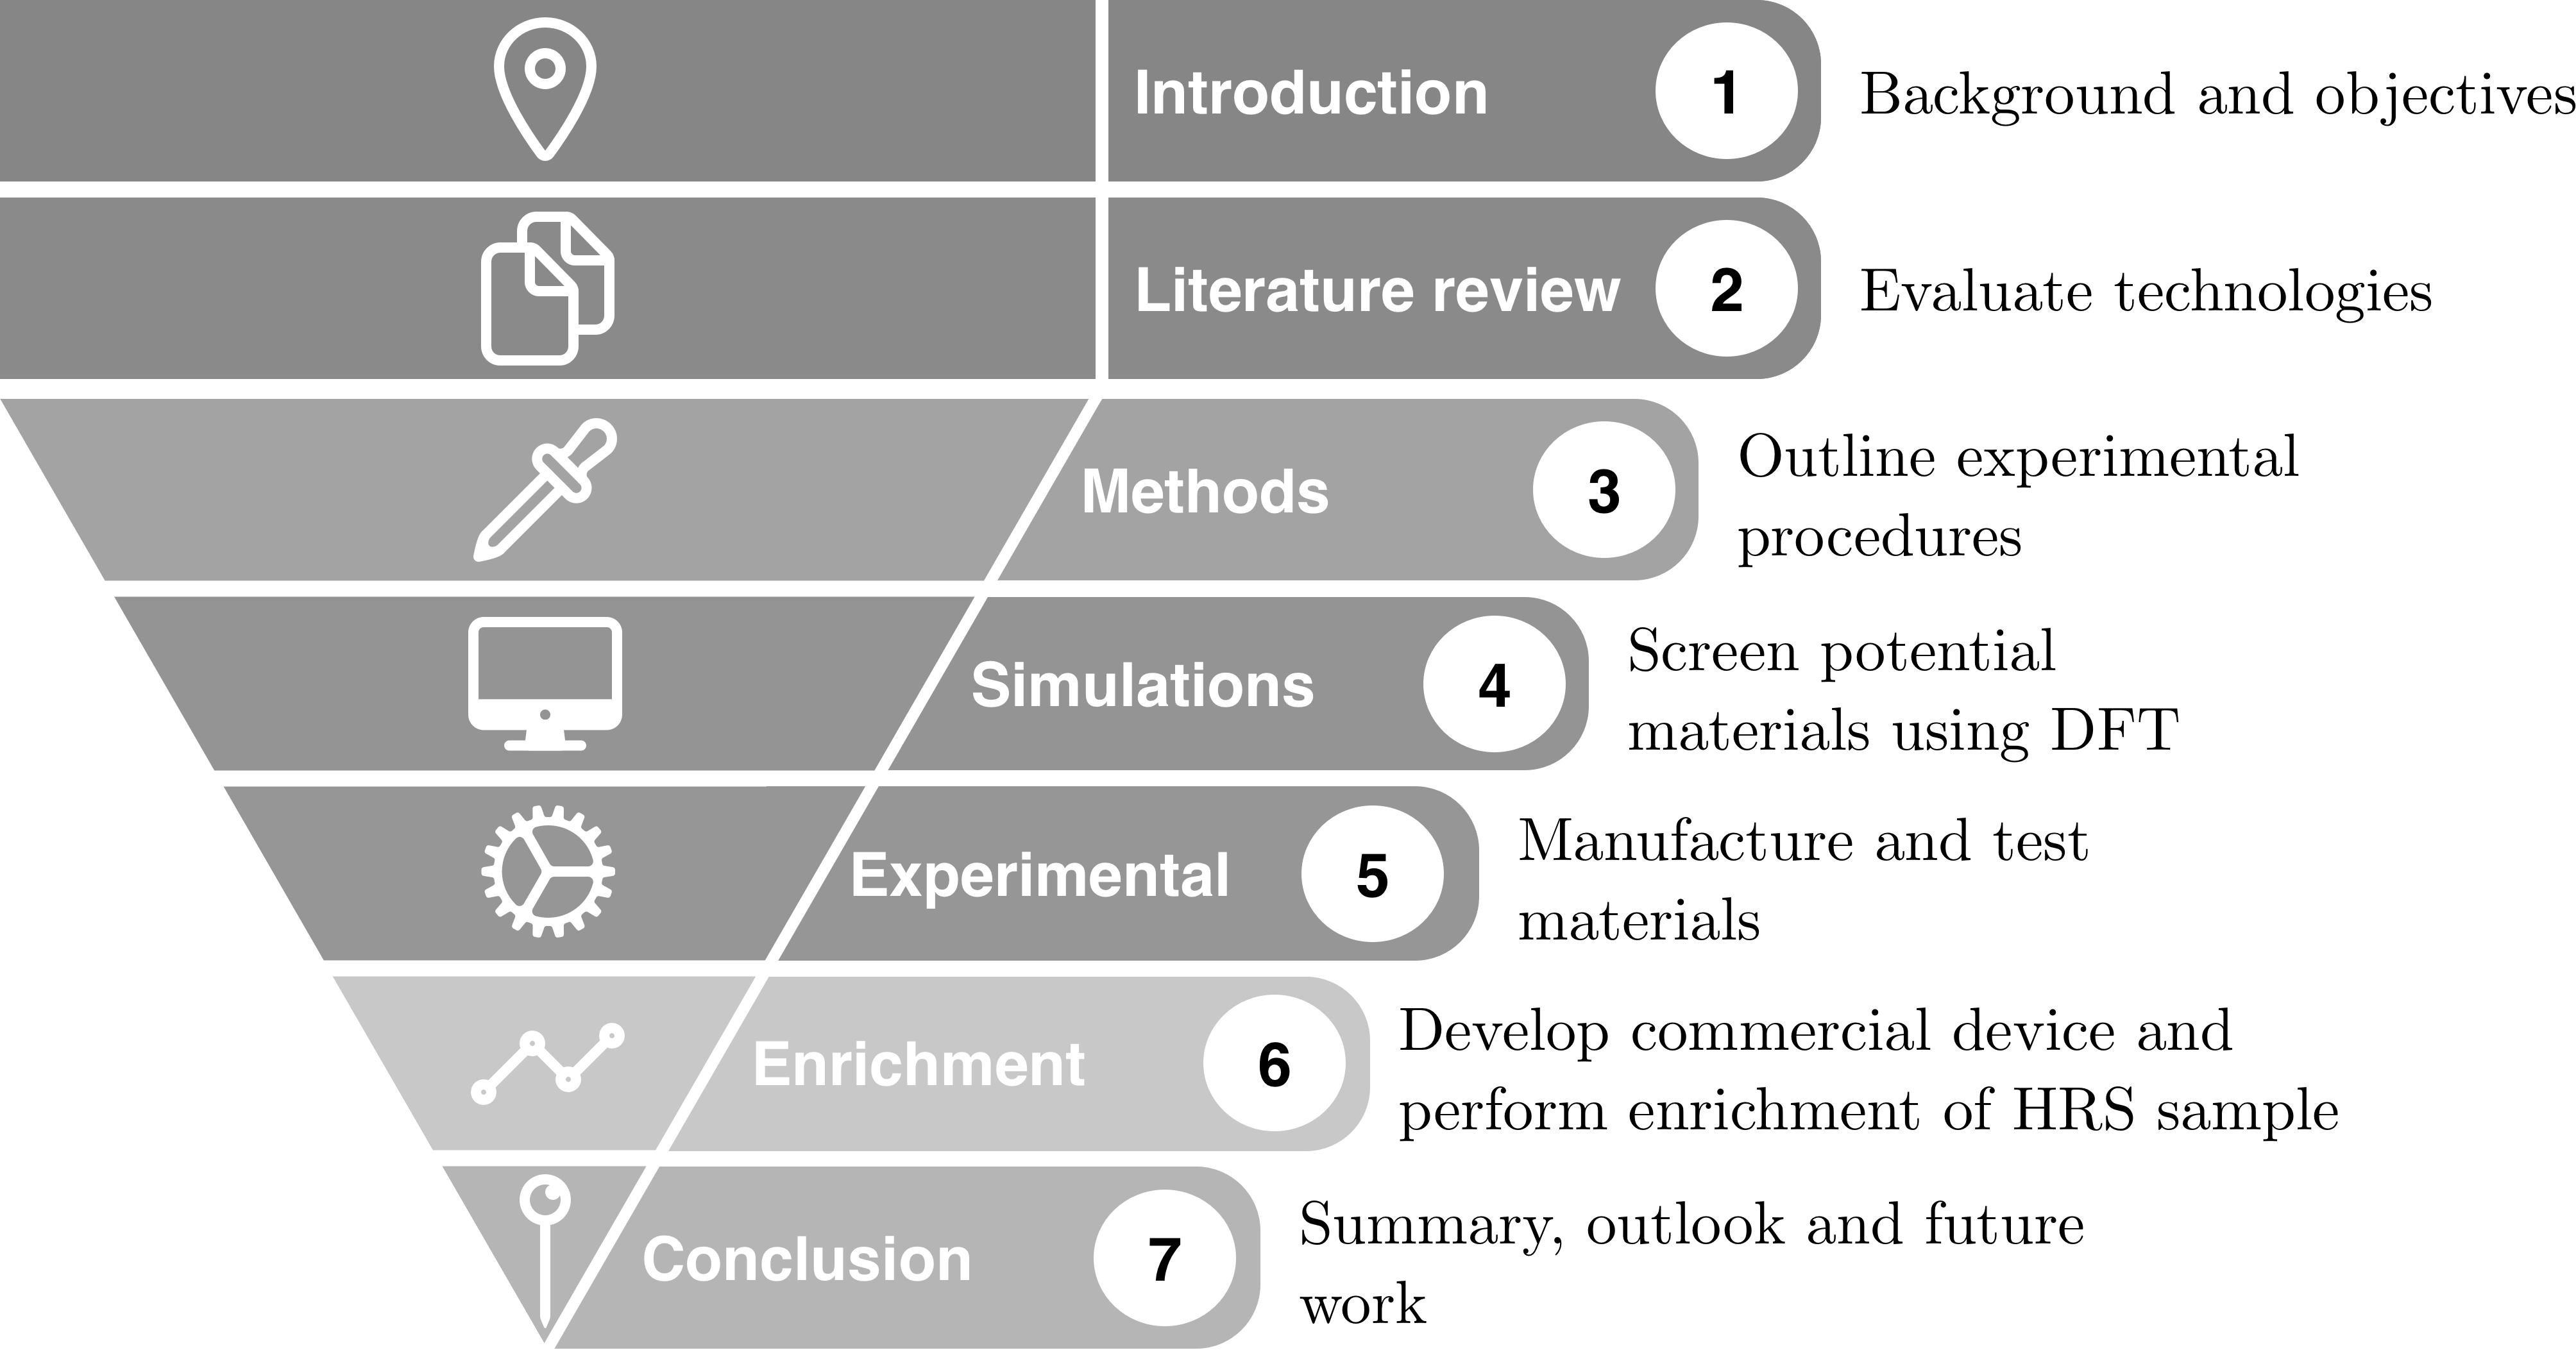
\includegraphics[width=\linewidth]{figures/funnel.png}
  \caption{Schematic presentation of the thesis structure}
  \label{fig:1}
\end{figure}


\renewcommand{\bibname}{References}
\bibliographystyle{unsrtnat}
\bibliography{library.bib}